\acresetall
\chapter{Background and Literature Review}
\label{ch:background}

\section{\ac{gps} \& \ac{waas} Introduction}\label{gps-waas-introduction}

The are numerous navigation aids supporting the national airways. Many
are ground based but with the inception of \ac{gps} there is a transition to space based navigation. In regards to utilizing \ac{gps} and \ac{waas} for navigation there are questions that need to be answered as to the necessity of \ac{waas} and why \ac{gps} by itself is not sufficient for aircraft navigation.

\begin{itemize}
\tightlist
\item
  Why yet another navigation system?
\item
  What are the benefits over other ground based navigational aids?
  \begin{itemize}
  \tightlist
    \item
      \ac{ndb}
    \item
      \ac{dme}
    \item
      \ac{vor}
    \item
      \ac{ils}
  \end{itemize}
\item
  What is \ac{waas}?
\item
  Why can \ac{gps} not be used on its own?
\item
  What does \ac{waas} do?
\item
  How does \ac{waas} work?
\item
  Where is \ac{waas} used?
\item
  Why use \ac{gps} and \ac{waas}?
\end{itemize}

\subsection{\ac{faa} Air Transportation System
Modernization}\label{faa-air-transportation-system-modernization}

The \ac{faa} has recognized the need to improve the Air Transportation System
so that it is more efficient, more predictable, and able to handle more
capacity while maintaining the highest safety standards and reducing
environmental impacts. The \ac{faa}'s NextGen modernization initiative is
geared toward moving away from ground-based to satellite-enabled
technologies for navigation and surveillance systems and from analog to
digital systems for communication. While \ac{waas} is not a NextGen program,
it is one of the foundational pillars upon which satellite enabled
technologies are built.

\subsection{Benefits of the Wide Area Augmentation
System}\label{benefits-of-the-wide-area-augmentation-system}

\subsubsection{Primary Means of
Navigation}\label{primary-means-of-navigation}

\ac{waas} is a critical component of the modernization's effort to enable the
aviation industry's use of space-based navigational aids as a primary
means of navigation, including: takeoff, en-route, approach and landing.

\subsubsection{More Direct Routes}\label{more-direct-routes}

Space-based navigational aids allows more direct routes to be utilized
over ground based navigational aids. It is not restricted by location of
ground-based equipment or line of sight as with some ground base
equipment. For example, utilizing \ac{vor}, which is a ground-based
navigational aid, is equivalent to navigating along a highway in the
sky. Using a \ac{vor} network, aircraft fly from one \ac{vor} to another which may
not be the most direct path. Utilizing \ac{gps} and \ac{waas} aircraft can fly
direct routes from their departure point to arrival point.

\subsubsection{Approach with Vertical Guidance
Capability}\label{approach-with-vertical-guidance-capability}

Additionally \ac{waas} approaches with
vertical guidance capability can be utilized at many airports for
landing. The number of airports that utilize \ac{waas} approaches has now exceeded that of airports using the
\ac{ils} which is another ground-based aid for landing
aircraft. The advantage of using \ac{waas} approaches as opposed to
\ac{ils} approaches is that \ac{waas} approaches do
not require ground-based equipment at the destination runways. The
infrastructure for an \ac{ils} requires antenna
arrays at the far end of the runway along with middle and outer markers
located along an established line-of-sight route to a destination
runway. The middle marker is 3000 to 6000 feet from the runway and the
outer marker is 4 to 7 miles. This is just for a single runway end. If
aircraft need to land from the opposite runway end all of this equipment
is duplicated and mirrored. The \ac{ils} infrastructure can be costly and
problematic and a full complement of equipment must be installed for
each runway end. Adding to the cost, an \ac{ils} needs its antennas and
markers routinely calibrated. It is an expensive installation, serves
only one runway end and requires ongoing calibration for each
installation.

\href{https://en.wikipedia.org/wiki/Marker_beacon}{ILS Marker Beacon}
{[}Link: NextGen Frequently Asked Questions{]}{[}1{]}\\
{[}Link: Performance Success Stories New WAAS Coverage Clears the Way
for New Access to Airports{]}{[}2{]}

Another deficiency is that it can just land aircraft, but it cannot
provide guidance for departures, missed approaches or any other
navigational service. If a missed approach is required the \ac{ils} cannot aid the aircraft on its outbound route. With
\ac{waas} a missed approach route can be defined. This is useful in areas
like Kodiak Alaska where the approach leads directly into the base of
Barometer Mountain; if a missed approach is required the pilot has to
bank hard left between the valley created by Barometer Mountain and Old
Women's Mountain. With the \ac{ils} or other
ground-based navigational aids rugged or mountainous terrain can make
line-of-sight systems unachievable. Space based navigation can have
issues in areas like urban canyons, but for aviation applications, space
based navigation has few impediments.

\href{https://www.google.com/maps/@57.7483115,-152.5265434,13z/data=!4m3!11m2!2s1o5YgbCjAjyBntt5HWecW-6ByCvg!3e3!5m1!1e4}{Kodiak
Alask Map}

Another benefit of \ac{waas} is that the ground-based infrastructure does not
have to be expanded to expand the capabilities of \ac{waas}. More approaches
can be added by surveying the runway ends and approach vector utilizing
\ac{gps} waypoints. The application is separate from the infrastructure. Just
as in \ac{gps} for vehicle navigation; \ac{gps} is providing positioning and
timing services and the applications of those services are ever
expanding.

\subsubsection{Decommission of Older, Expensive Ground-Based Navigation
Equipment}\label{decommission-of-older-expensive-ground-based-navigation-equipment}

As satellite navigation systems become the primary means of navigation
and supplants those capabilities of older ground-based navigational aids
those aids can be decommissioned. As more approaches are defined more
\acp{ils} can be the decommissioned. As direct en-route capabilities are
established the \ac{ndb}, \ac{dme} and \ac{vor} systems can also be decommissioned.

\href{https://www.uasc.com/docs/default-source/documents/universalflyer/uasc_universalflyer_20122q.pdf?sfvrsn=e717985c_2}{FAA
Announces Plan for Reduction in VOR and ILS in Favor of WAAS}

\subsubsection{Simplified Avionics}\label{simplified-avionics}

With the implementation of \ac{waas} and \ac{laas}, as currently planned by the \ac{gps} Product Team, a substantial reduction in the user avionics equipment cost can be realized because of the reduction in the proliferation of navigational devices. A single device can serve all phases of flight.

\href{https://www.faa.gov/about/office_org/headquarters_offices/ato/service_units/techops/navservices/gnss/library/satnav/media/SatNavNews_Summer_2017.pdf}{The
Sum of All Performance-Based Navigation Procedures}

\subsubsection{Increased Capacity}\label{increased-capacity}

\ac{waas} enabled receivers provide a highly accurate \ac{gps} position solution,
so an aircraft's position is known to a higher fidelity than has
previously been available. This, along with other technologies being
pursued by the \ac{faa}, will offer opportunities to reduce separation
standards. This reduction will be an incremental process based on
analysis of the evolving capabilities. Potential reductions include
non-radar separations in en route airspace and terminal separations due
to smaller obstacle clearance areas and protected airspace. Reduced
separation standards will directly translate into increased system
capacity that can safely fly in a particular volume of airspace,
benefiting the aviation user community.

\href{https://www.faa.gov/about/office_org/headquarters_offices/ato/service_units/techops/navservices/gnss/library/satnav/media/SatNavNews_Spring2014_final_web.pdf}{WAAS
Benefits Driving Equipage}

\subsubsection{Resiliency}\label{resiliency}

\ac{waas} does require a ground-based equipment infrastructure, but that
infrastructure is highly resilient and redundant and \ac{waas} enabled
applications can be implemented with no need to expand \ac{waas}
ground-based equipment. It has a dual ring active/active network along
with active standby and backup equipment. If an outage happens with any
one piece of \ac{waas} equipment it can be placed in standby mode until such
time as it is appropriate to send maintenance personnel to work on it.
This is different from the \ac{ils} or \ac{vor}
systems, where if that ground-based navigational aid has a malfunction,
that service is rendered unavailable until the repairs are completed.
Depending on the criticality of the system, \ac{faa} maintainers may need to
be out in the field in adverse weather conditions to restore service.
Some equipment locations, like Kotzebue, Alaska, are inhospitable most
of the year, so it makes it very precarious for maintainers to get out
to those facilities to restore equipment and services. For \ac{waas}, a loss
of a subsystem does not mean a loss of service. Though it is not
optimal, with the redundancy build into \ac{waas} ground-based equipment
infrastructure it can run in a degraded state with no system impact
until conditions are suitable for the restoration.

\subsection{\ac{gps} Overview}\label{gps-overview}

\ac{waas} is a space-based differential \ac{gps} system. It is used to detect and
correct \ac{gps} errors, monitor and correct for ionospheric delay and also
provides additional ranging sources from three GEO satellites for
improved availability of space based navigation services. It augments
\ac{gps} and improves accuracy, integrity, and availability. At its core \ac{waas}
is a real-time \ac{gps} sensor network. To understand why \ac{gps} can't be used
by itself, how \ac{gps} operates needs to covered. \ac{gps} works by determining
the range from the \ac{gps} satellite to the user receiver. With one \ac{gps}
satellite the user knows that he is on the sphere from the \ac{gps} satellite
to the receiver. The user can be located anywhere on the surface of the
sphere created by the range of the satellite to the user receiver.
Introducing another \ac{gps} satellite, the user can now be isolated to the
intersection of two spheres which is a circle. With a third satellite
the user is at the intersection of three spheres which is two points.
\ac{gps} assumes an earth centered, earth fixed,
x-y-z 3D Cartesian coordinate system. Any location in this 3D space
requires no more than 3 components to be completely identified. So, even
though the intersection of 3 spheres yields two different points, the
point located outside the earth's atmosphere is rendered useless by the
earth centered earth fixed reference system. One point will be within
Earth's atmosphere with an acceptable rate of velocity while the other
point will be in space traveling at a high velocity.

If the user measurements were perfect then three satellites would be
sufficient to determine the user's location, but to take near perfect
measurements would require the use of a highly stable atomic or optical
clock. These clocks are large, very expensive and require considerable
power, so the use of these types of clocks is impractical. Most \ac{gps}
receivers utilize a quartz crystal oscillator for timing. This
oscillator is small, cheap and low power but also very inaccurate, but,
as it turns out, if three perfect measurements can locate a point in
3-dimensional space, then four imperfect measurements can do the same
thing. \ac{gps} utilizes a fourth satellite to solve for the user's clock,
synchronizing the receiver clock with \ac{gps} time. Since any offset from
\ac{gps} universal time will affect all of the measurements, the receiver
looks for a single correction factor that can be subtract from all its
timing measurements that would cause them all to intersect at a single
point. That correction brings the receiver's clock back into sync with
\ac{gps} time. The fourth satellite helps calculate the timing correction and
in turn a location correction and selects one of the remaining two
points as the position. The fourth satellite allows for the solving of a
linear set of equations for x, y, z, and t simultaneously. Four
satellites are required for (x,y,z,t) but in normal operation users are
tracking more than four satellites; typically around 6 to 8. This sets
up an overdetermined system of equations and a least-squares algorithm
is used to determine the minimum error position solution. An added
benefit is that every \ac{gps} receiver essentially has atomic-accuracy.

{[}Link: Getting Perfect Timing Using \ac{gps} for Timing{]}{[}3{]}\\
{[}Link: Trilateration algorithm for n amount of points{]}{[}4{]}

\section{\ac{gps} Overview}

The \ac{gps} is a remarkable system for finding one's location and its success is largely due to the modest needs of the average user. Standard \ac{gps} accuracy is approximately 15 meters\citep[]{GPS_FOR_DUMMIES} and this level of accuracy is quite satisfactory for many applications, including land navigation, which is the primary consumer application for \ac{gps}. However, when \ac{gps} accuracy is discussed it is generally in terms of horizontal accuracy.  Vertical accuracy is seldom mentioned in the discussion of accuracy and most \ac{gps} manufacturers do not publish the vertical accuracy specification.  Due to this, a rule-of-thumb has developed that suggests that the vertical accuracy is only half as good as the horizontal accuracy.  So, if Standard \ac{gps} is accurate to within 15 meters in the horizontal, then it is considered accurate to about 30 meters in the vertical, which is unacceptable for aircraft landings. This is why \ac{laas} is indispensable for a \ac{gls}.  Many different factors affect the precision of \ac{gps} which will be explored during this overview of \ac{gps}.

\ac{gps} is comprised of 24 well placed satellites. The satellites orbit the earth in 6 orbital planes that are at a 55$^o$ inclination with 4 satellites per plane such that at least 4 satellites will be above the horizon at any given moment. This allows users the ability to use the system 24 hours a day anywhere on the planet. These satellites are not geo-orbital, but are at a \ac{meo} and orbit the earth twice a sidereal day with a speed of 3.9km per second.  The basic principal of the \ac{gps} system is quite simple.  A satellite orbits the earth at about 12,600 miles shown in Figure~\ref{fig:GPS_Basics_1}. The satellite acts as a reference point with a known distance which is called its \textit{range}.  How this range is known will be discussed later, but for now the user receiver knows one thing, that it lies on a sphere centered at the satellite with a known radius.

\begin{figure}
  \centering
	\scalebox{.9}{
	\mbox{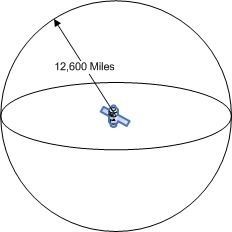
\includegraphics{figures/GPS_Basics_1.jpg}}
	}
  \caption{\ac{gps} Basics: Radius}
	\label{fig:GPS_Basics_1}
\end{figure}

If two satellite are used then this narrows the possible location down to the circle where the two spheres centered at each satellite intersect, shown in Figure~\ref{fig:GPS_Basics_2}. When a third satellite is introduced it intersects the circle at two points shown in Figure~\ref{fig:GPS_Basics_3}. Purely speaking a fourth measurement should be used to unambiguously locate a point in space, but for \ac{gps} this is not the case.  Of the two points referenced, one is normally a sensible answer and the other is either not located on Earth or is moving at an unreasonable velocity (measured in the range of thousands of kilometers per second).

\begin{figure}
	\centering
	\scalebox{.5}{
	\mbox{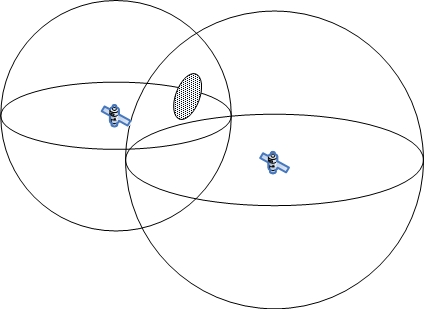
\includegraphics{figures/GPS_Basics_2.jpg}}
	}
	\caption{\ac{gps} Basics: Circle}
	\label{fig:GPS_Basics_2}
\end{figure}


\begin{figure}
	\centering
	\scalebox{.55}{
	\mbox{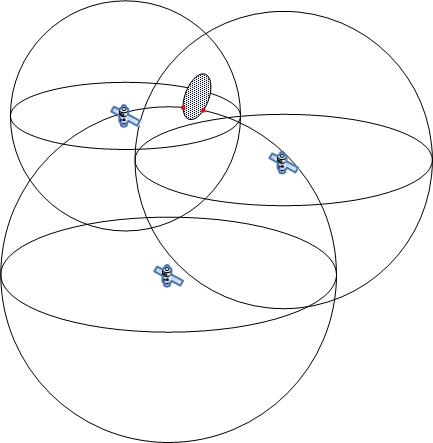
\includegraphics{figures/GPS_Basics_3.jpg}}
	}
	\caption{\ac{gps} Basics: Two Points}
	\label{fig:GPS_Basics_3}
\end{figure}

The satellites are used as reference points, but how can something moving high above the earth at a high velocity be used for measuring distance?  Every aspect of the \ac{gps} constellation is precisely monitored by six earth based monitor stations located throughout the world.  Any variance in the orbit, position, or velocity of a satellite is compensated and adjusted for at the master control station, located in Colorado Springs, Colorado.  These constant adjustments are put into a \ac{gps} message called the ephemeris message.  An \textit{ephemeris} is a table giving the coordinates of a set of celestial bodies at a number of specific times during a given period.  This data allows a \ac{gps} receiver to know the exact position of a satellite at a given time.  Now a method similar to \textit{trilateration} can be used to determine the \ac{gps} receiver's range or distance to the satellite. Trilateration uses the known locations of three or more reference points, and the measured distance between the subject and each reference point to determine the subject's location. In the case of \ac{gps} the distance is measured using the \ac{toa} of a ranging signal called the \textit{pseudorandom code}. The code is a very complex set of digital information that is called pseudorandom because it resembles random noise. It is repeated every millisecond. When the receiver receives the pseudorandom code it takes the signal propagation time multiplied by the speed of light to get the range to the satellite.  This is simple in concept, but the timing has to be near perfect.  If the time is off by even 1/1000 of a second the range could be off by 300,000 meters.  The satellites actually keep track of time using atomic clocks.  Each satellite is equipped with four atomic clocks to precisely track time, but atomic clocks are very costly and impractical for producing low cost \ac{gps} receivers.  Instead manufacturers use a less precise, less expensive crystal clock; but now have to overcome the error introduced by the receiver clock. Thus time becomes a fourth unknown. This is resolved with an additional satellite measurement. If three measurement made with perfect time can be used to produce a position solution then four inexact measurements can be used to produce the same solution while solving for the receiver clock offset.  Once the receiver's clock has been adjusted then not only will the receiver produce an accurate position, but it also works as a functional atomic clock.  Theses techniques provide a more accurate range to satellites, but these ranges still contain errors; therefore they are referred to as \textit{pseudoranges}.  The errors can be categorized as follows:

\begin{itemize}
	\item Ephemeris ($<$ 1 meter Error)

As mentioned earlier an ephemeris is a table of the coordinates of a celestial body at a point in time. This of course uses a model to predict where the satellite will be, but the forces acting upon the satellite don't always conform perfectly to the model which does introduce some error.  Since the ephemeris data is constantly being adjusted the error introduced is small and can be removed by differential \ac{gps} between two observations of short separation.

	\item Satellite Clock Errors ($<$ 1 meter Error)

Satellites use atomic clocks to precisely monitor time, but even atomic clocks are not perfect.  Since the pseudorange calculation is based on time any discrepancy in the clock will introduce error.  This can also be removed with differential \ac{gps}.

	\item Receiver Clock Errors (1 meter $<$ Error $<$ 2 meters)

A \ac{gps} Receiver uses a crystal clock which is much less accurate than an atomic clock; consequently additional timing errors exist.  The Receiver Clock produces more error than the Satellite Clock and unfortunately can not be removed with differential \ac{gps}, but is treated as another unknown during the estimation process.

	\item Ionosphere / Troposphere ($\approx$4 meters)

The atmosphere can be broken down into many layers but the two that most affect \ac{gps} are the Ionosphere and the Troposphere.  The Ionosphere is a dispersive medium, therefore the \ac{gps} signal is bent and changes speed as it passes through the ionosphere. Though the bending is generally negligible, the ionosphere increases the speed of the carrier phase and slows down the pseudorandom code, so this source of error must be taken into consideration.  The troposphere, on the other hand, is a non dispersive medium, so the carrier phase and pseudorandom code are delayed by the same amount increasing the measured distance to the satellite from the actual distance.\cite[]{EL-RABBANY}.

 	\item \ac{gps} Satellite Geometry

A Satellite's geometry with respect to other satellites also plays a role in the position solution.  The closer the satellites are to one another the poorer the position solution and the more spread out the better the position solution.  The \ac{dop} is a number that represents the acceptability of the \ac{gps} geometry.  It can further be broken down into a horizontal and vertical component known as the \ac{hdop} and \ac{vdop}.

	\item Multipath

Multipath is a source of error that is introduced when the \ac{gps} signal is received by the \ac{gps} receiver from different paths; one signal may take the direct path and another signal be reflected off of some structure. This is the same occurrence that causes ghosting on a television set. \ac{laas} reduces the potential of this error source by using specialized \ac{gps} \acp{mla} and a priori siting analysis to avoid multipath generating structures.

	\item \ac{sa} ($>$ 10 Meters)

The last error that will be mentioned is artificial error.  The U.S. Military purposely skewed the \ac{gps} signal to artificially inflate the error in the system so that it could not be used against them.  When \ac{sa} was active it was the most substantial source of error, but the use of differential \ac{gps} could nearly eliminate \ac{sa}'s effectiveness. The use of \ac{sa} was discontinued on May 1, 2000.

\end{itemize}

\section{\ac{dgps}\label{section:DGPS}}

\ac{dgps} is the method of using a \ac{gps} receiver at a fixed known reference point to determine the errors in \ac{gps} ranging. To do this, the \ac{gps} receiver's antenna position is accurately surveyed.  Next, the difference is calculated between the pseudorange internally measured by the \ac{gps} receiver and the pseudorange calculated from a satellite's current \ac{gps} almanac, ephemeris information, and the surveyed location.  The difference between the measured pseudorange and the calculated pseudorange is the \textit{pseudorange correction} which is the distance that the local user should adjust a respective satellite's pseudorange by to achieve a minimum error position solution. The pseudorange correction is a lump sum adjustment for multiple sources of error which include ephemeris, satellite and receiver clocks, ionosphere and troposphere, and even Selective Availability. However, the pseudorange correction can only be computed by knowing the precise location of the reference receiver antenna. Another thing to note is that most \ac{dgps} systems make corrections in the range domain by adjusting the pseudorange measurement of each satellite in view.  An alternative approach is to adjust the system in the position domain.  This would involve calculating a position solution for the reference point then calculating a position correction vector.  This is generally not done due to the fact that position solutions are calculated by manufacturers using proprietary methods, and their behavior is not known a priori.

The many different \ac{dgps} solutions that have been developed fall broadly into two categories: post-processed and real time. Surveyors are a primary user of the non-real time post-processing category.  They collect \ac{gps} data from known reference points, which they call \textit{benchmarks}, and the point needing to be surveyed.  The distance between the benchmark and the survey point is called the \textit{baseline}, and it is generally preferred to use the benchmark with the shortest baseline to the survey point. After about 15 minutes to an hour of collecting data at both locations they can post process the data with \ac{gps} utilities to produce a position solution accurate to within a centimeter\footnote{Utilizes \ac{gps} L1/L2 survey equipment}.  On the other hand, real-time differential \ac{gps} systems acquire the data from the reference points, calculate the pseudorange corrections, and broadcast them out at a rate of 2 to 5 Hertz to be used in navigation applications. Since \ac{laas} falls into the real time category, it and a few other prominent real time \ac{dgps} systems will be discussed.

One of the first systems developed actually used the acronym \ac{dgps}, but sometimes also goes by \ac{ndgps} to distinguish \ac{dgps} the concept from \ac{dgps} the system.  The \ac{ndgps} is used by the U.S. Coast Guard in harbor regions to give ships better position solutions.  Even though the name implies national coverage is it limited to coastal regions. Europe and Canada also have similar solution for their heavily utilized maritime locations. There are even commercial companies like VERIPOS, StarFire, and OmniSTAR that provide \ac{dgps} services.

\begin{figure}
	\centering
	\scalebox{1.437}{
	\mbox{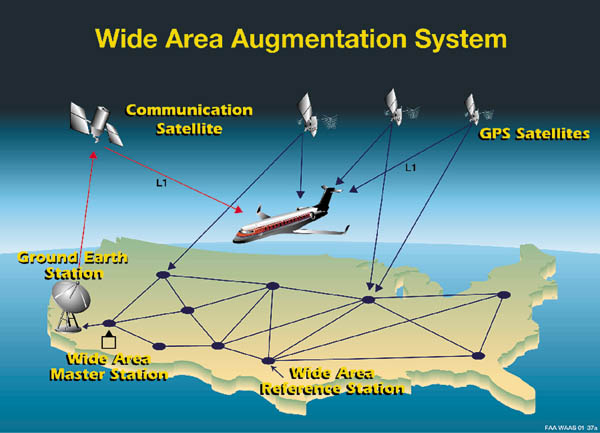
\includegraphics{figures/waas.jpg}}
	}
	\caption{Wide Area Augmentation System\citep[]{FAA_WAAS}}
	\label{fig:FAA_WAAS}
\end{figure}

Most of the \ac{dgps} systems developed had a very specific function or operated in such a localized area that it precluded widespread use. The \ac{faa} wanted to capitalize on the benefits of \ac{dgps} while promoting a broad coverage area. To that end they designed \ac{waas}, as shown in Figure~\ref{fig:FAA_WAAS}, established reference points throughout the contiguous United States. These fixed reference points were used to establish pseudorange corrections for most of North America.  \ac{waas} corrections are then sent to a geo-orbital satellite and broadcast to \ac{waas}-enabled \ac{gps} receivers.  \ac{waas} improved the accuracy of \ac{gps} to less than 2 meters in the horizontal and less than 3 meters in the vertical. This was a significant enhancement to \ac{gps}; an improved \ac{gps} position solution free for the end user.  \ac{gps} manufacturers adopted this readily and now \ac{waas}-enabled \ac{gps} receivers are commonplace. A major shortcoming with \ac{waas} is its confinement to North America.  Additional Reference Receivers are being installed in Alaska and Mexico, but this is still a United States / North America locale. Large air carriers need \ac{gps} augmentation internationally. Furthermore, \ac{waas} accuracy is not as accurate as some other \ac{dgps} systems due to its broad coverage area.  Because of this the \ac{faa} does not consider its accuracy and integrity acceptable for instrument landings beyond CAT I.

\begin{figure}
	\centering
	\scalebox{.907}{
	\mbox{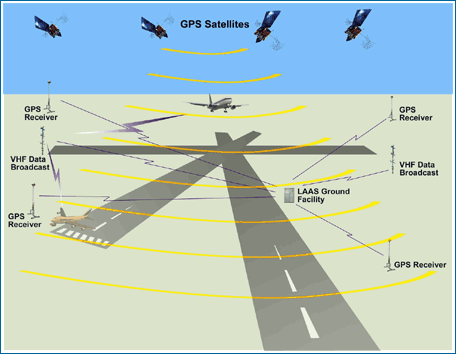
\includegraphics{figures/LAAS_Architecture.png}}
	}
	\caption{Local Area Augmentation System}
	\label{fig:FAA_LAAS}
\end{figure}

\subsection{Why can't you use \ac{gps} by
itself?}\label{why-cant-you-use-gps-by-itself}

\ac{gps} has many errors associated with it and due to these errors the \ac{gps}
signal does not meet the accuracy, integrity, availability, and
continuity requirements critical to safety of flight. Clock errors,
ephemeris errors, errors in the troposphere, errors in the ionosphere
and multipath errors each cumulatively reduce \ac{gps} accuracy. \ac{waas} is an enhancement to \ac{gps} which monitors
and detects these associated errors and provides the necessary
corrections for meeting safety-of-life flight requirements. The purpose
of \ac{waas} is to monitor the \ac{gps} constellation and detect and correct for
errors when possible. If corrections are not possible \ac{waas} will alert
aviation users when \ac{gps} services cannot be used; the most notable being
ionospheric storm events where changes in the ionosphere are changing
too rapidly for the \ac{waas} ionoshperic model to adapt. \ac{waas} is able to
detect errors by utilizing a robust ground-based geographically diverse
sensor network. There are 38 \ac{waas} reference stations dispersed
throughout Alaska, Canada, continental US, Mexico and Hawaii. Each
reference station has three \ac{gps} receivers who's location coordinates are
precisely surveyed. Errors in the \ac{gps} signal can be detected and these
errors are grouped into two different classes; the \ac{udre} and the Grid Ionospheric Vertical Error. One is a per \ac{gps}
satellite based correction and the other is a geographical based
correction to account for the delay of the \ac{gps} signal through the
ionosphere. How this works for the end user is that their avionics
receiver calculates a protection level. If their protection level is
within the alert limits specified in the \ac{waas} \ac{mops} then \ac{waas}
services available for them and they can utilize \ac{waas} corrections to
increase their accuracy. If however, they calculate a protection level
that is outside the alert limit then \ac{waas} is unavailable for them and
they can not use the \ac{waas} service. There exist a case that a protection
level is calculated and it is within the alert limit but the true
position of the aircraft is outside of those boundaries. This is the
situation where the user determined they are safe when they are not.
This is called Hazardously Misleading Information (HMI). This is an area
in which National Airways System Engineering spends considerable time
evaluating to ensure users are protected.

Along with the user clock error there are other \ac{gps} error sources that
affect the utilization of \ac{gps}. There could be errors with the clock
onboard the \ac{gps} satellite itself. There is also error in the ephemeris
message. The ephemeris is a mathematical models of the motion of the
orbit of a satellite. This orbit model is provided to the user and any
errors in the model will add to a user's position error. Temperature,
pressure and humidity in the troposphere, the lowest layer of the
Earth's atmosphere, can also affect a \ac{gps} signal's propagation. A
significant source of propagation delay is the ionosphere. The
ionoshpere is the ionized part of Earth's upper atmosphere and can
contribute anywhere from 10 to 30 meters of error. The last source of
error is multipath. Multipath is caused when a signal is reflected from
surfaces near the receiver's antenna, such as buildings, and the
reflections are mistaken for the primary signal. The reflected signal
adds additional propagation delay over the true signal, and in turn,
additional user error.

\ac{waas} has mitigations and corrections for each type of error. First, \ac{waas}
mitigates the user clock error by using cesium atomic clocks. This is a
highly stable and accurate time source that disciplines the clock of the
\ac{gps} receiver used by the \ac{waas} reference station. It mitigates multipath
interference by using a highly specialized multipath limiting antenna.
\ac{waas} has an orbit determination filter to minimize the ephemeris errors
of \ac{gps} and GEO satellites. \ac{waas} also utilizes a Kriging model for the
ionosphere and provides ionospheric corrections for all of North
America. By mitigating the error sources in the acquisition of the \ac{gps}
measurement data, \ac{waas} is able to detect \ac{gps} errors and provide corrects
for those errors to users to increase their accuracy.

\subsection{What is \ac{waas}}\label{what-is-the-wide-area-augmentation-system-waas}

\ac{waas} is a space-based differential
\ac{gps} system. It detects and corrects \ac{gps} errors, monitors and corrects
for ionospheric delay and provides additional ranging sources for
improved availability of the navigational service. It augments \ac{gps} and
improves its accuracy, integrity and availability. At its core \ac{waas} is a real-time sensor network and the
sensor is a \ac{gps} antenna tracking all \ac{gps} satellites in view of that
antenna.

\subsection{What is the purpose of
\ac{waas}?}\label{what-is-the-purpose-of-waas}

\ac{waas} is designed to protect users from error sources and other threats
inherent in using \ac{gps}. It does this by broadcasting a \ac{udre}, a \ac{give} and \ac{gps}
health information to the user. \ac{waas} has predefined alert limits fixed
by specification. The aircraft's \ac{waas} enabled avionics will calculate
its \ac{gps} position while applying the \acp{wum} which have the
\ac{udre} and the \ac{give} values. The avionics receivers use these values to
calculate a protection level based on the algorithm specified in the
\ac{waas} \ac{mops}. If its protection level is within the alert limits then \ac{waas}
is available for that user. If it calculates the protection level and it
is beyond the alert limit then \ac{waas} is not available for that user. If
the protection level cylinder becomes too small and does not enclose the
true position of the aircraft this is called hazardously misleading
information. It is a scenario in which the calculated protection level
misinforms the user that the system is available for them to use when it
is not.

\subsection{How does \ac{waas} work?}\label{how-does-waas-work}

\subsubsection{\ac{wrs}}\label{waas-reference-stations}

The \ac{gps} satellites broadcast their ranging signal and message data down
to earth and it is collected at a 1Hz rate by a network of \ac{wrs}. There are 38 reference stations that are
geographically diverse across North and Central America including
Alaska, Canada, Continental US, Mexico and Hawaii. Each reference
station has three threads denoted as thread A, B and C, so 114
individual threads. The A and B threads of each reference station are
primarily utilized and the C thread is an active standby. A \ac{wrs} can
withstand an outage from any one thread. In fact \ac{waas} can withstand the
outage of one or more complete reference stations as long as they are
not in close geographical proximity to on another. If multiple reference
stations are out of service in a local area this will impact the
ionospheric model and coverage will be reduced or lost in that area. \ac{gps}
measurement data from every \ac{gps} satellites being tracked by all 114
threads is put onto a high availability terrestrial communications
network. The network connects the reference stations to the \ac{wms}.

\subsubsection{Wide-Area Master Station (WMS)}\label{waas-master-stations}

There are three \ac{wms} that pull in the \ac{wrs} data and
calculate the differential \ac{gps} corrections, ionospheric correction and
validates the \ac{gps} satellites are operating in a healthy normal mode. If
a satellite is not usable \ac{waas} will send a \ac{dnu} alert
message out to the users. These master stations are what calculate all
the integrity parameters and is the computational center point of the
system. The software for all the integrity monitors is running on a
real-time operating system and is maintained using the guidelines
specified in DO-178B, Software Considerations in Airborne Systems and
Equipment Certification up to a Software Level of B/Hazardous. Once all
the integrity parameters, the corrections and health information are
validated and calculated the information is formulated into a series of
\acp{wum} and then put on the terrestrial communications
network and sent to the \ac{gus}.

\subsubsection{GEO Uplink Subsystem}\label{geo-uplink-subsystem}

\ac{waas} has three GEO satellites. Each satellite has two uplink stations
denoted as primary and backup. The denotation for each system is based
on which station is radiating to the satellite. The \ac{gus}
that is radiating to the satellite is designated as primary and the
other, which is radiating into a dummy load, is denoted as backup. If
for some reason the primary has a failure it will automatically switch
to the backup and the backup will become primary. When the faulted GEO
Uplink Subsystem is restored to service it will be brought up into
backup mode. It will stay in backup mode until the primary faults and
automatically switches over back to primary or the \ac{waas} operator issues
a command to initiate a manual GUS switch over. This is done for
maintenance activities at GUS sites.

The \ac{gus} sends the \ac{wum} through the \ac{rfu} which broadcast it to the \ac{waas} satellite in
geosynchronous orbit. The \ac{waas} GEO satellite broadcasts the differential
and ionospheric corrections as well as \ac{gps} satellite heath back down to
the aviation users. The avionic equipment applies the \ac{waas} corrections
to increase the accuracy of its \ac{gps} position solution. \ac{waas} provides
another service called GEO Ranging. The three \ac{waas} GEO satellites
provide a ranging signal that functions like a \ac{gps} signal. These
additional ranging sources help fill in the usable satellite
constellation and also provides better satellite geometry. This
increases the availability of using space based navigation services
because the \ac{gps} constellation has now been augmented with three
additional satellites. If a \ac{gps} satellite is taken out of service the
three \ac{faa} GEO ranging satellites will help fill in the constellation.
The geometry of the satellite constellation has values associated with
it called the dilution of precision. The more dispersed the
constellation the better its dilution of precision. The more tightly
grouped the satellite constellation is the worse the dilution of
precision. The better dilution of precision value the better the
position solution will be.

{[}Link: Dilution of Precision{]}{[}5{]}

\subsubsection{Operation and Maintenance
System}\label{operation-and-maintenance-system}

The \ac{waas} system has two operation and maintenance systems located in
Warrenton, VA and the other in San Diego, CA. This is where the \ac{waas}
operators monitor and control the \ac{waas} system.

\subsection{Where is \ac{waas} used?}\label{where-is-waas-used}

\ac{waas} currently uses three geosynchronous satellites with a footprint
that covers the entire Western Hemisphere. Coverage over the northern
slope of Alaska is particularly valuable to the \ac{faa} due to Alaska having
many general aviation users that utilize \ac{waas}. As of May 24, 2018, there
are 3,909 \ac{waas} Localizer Performance
with Vertical guidance (LPV) approach procedures serving 1,900 airports.
1,138 of these airports are Non-\ac{ils} airports. Currently, there are also
661 Localizer Performance (LP) approach procedures in the U.S. serving
495 airports.

{[}Link: Satellite Navigation - GPS/WAAS Approaches{]}{[}6{]}

\begin{center}\rule{0.5\linewidth}{\linethickness}\end{center}

\section{Items to look into:}\label{items-to-look-into}

One significant improvement \ac{waas} provides is the elimination of
errors for hot and cold temperatures that previously affected baro type
vertical navigation systems. \ac{waas} equipped receivers will automatically
notify the pilot of the most accurate level of service provided for that
given receiver, signal, and approach.

One significant difference between satellite based navigation as opposed
to ground based is that distances: Are given Along Track Distance (ATD)
during the final approach segment.

One primary difference between an RNAV approach with \ac{gps} and \ac{waas} is at
the missed approach point \ac{gps} suspends while \ac{waas} sequences to the
missed approach procedure.

\begin{center}\rule{0.5\linewidth}{\linethickness}\end{center}

The \ac{faa} will seldom, if ever, install a new \ac{ils}, opting instead for PBN
landing procedures, which save money. Further costs saving are gained by
reducing the existing ground-based navigation infrastructure, which
remains as a backup in case of disrupted satellite service. {[}1{]}:
https://www.faa.gov/nextgen/faqs/ {[}2{]}:
https://www.faa.gov/nextgen/snapshots/stories/?slide=5 {[}3{]}:
http://www.trimble.com/gps\_tutorial/howgps-timing2.aspx {[}4{]}:
https://gis.stackexchange.com/questions/40660/trilateration-algorithm-for-n-amount-of-points/40678\#40678
{[}5{]}:
https://en.wikipedia.org/wiki/Dilution\_of\_precision\_(navigation)
{[}6{]}:
https://www.faa.gov/about/office\_org/headquarters\_offices/ato/service\_units/techops/navservices/gnss/approaches/

https://www.faa.gov/about/office\_org/headquarters\_offices/ato/service\_units/techops/navservices/gnss/faq/gps/?iframe=true\&width=100\%\&height=100\%
Q. Is the basic \ac{gps} signal sufficient to meet all the needs of civil aviation?

A. This is not a simple yes/no answer. The answer is that it depends on
the service requirements of each user or aviation authority. For many
countries, \ac{gps} supplies a better capability than the existing
ground-based systems or lack thereof. Yet for other countries with large
infrastructures, the \ac{gps} signal does not meet the accuracy, integrity,
availability, and continuity requirements critical to safety of flight.
Enhancements to the \ac{gps} such as \ac{waas} and \ac{gbas} provide the necessary corrections for meeting safety-of-life flight requirements.

\begin{sidewaystable}[htbp]
\centering
\caption{\ac{waas} Sites}
\resizebox{\columnwidth}{!}{
\begin{tabular}{ l l l l l}
\hline
\textbf{City} &
\textbf{ICAO airport code} &
\textbf{Antenna 1} &
\textbf{Antenna 2} &
\textbf{Antenna 3}\\ \hline
Bethel, Alaska                           & PABE     & 60.787916486°N 161.841724416°W, 52.203 m    & 60.787897064°N 161.841663857°W, 52.204 m    & 60.787881127°N 161.841728605°W, 52.198 m\\
Billings, Montana                        & KBIL     & 45.803707088°N 108.539722283°W, 1112.261 m  & 45.803716383°N 108.539780649°W, 1112.266 m  & 45.803756811°N 108.539680968°W, 1112.255 m\\
Barrow, Alaska                           & PABR     & 71.282765883°N 156.789923397°W, 15.577 m    & 71.282798595°N 156.789965306°W, 15.589 m    & 71.282793925°N 156.789856228°W, 15.577 m\\
Cold Bay, Alaska                         & PACD     & 55.200334771°N 162.718472052°W, 53.648 m    & 55.200394330°N 162.718489390°W, 53.652 m    & 55.200400493°N 162.718623936°W, 53.657 m\\
Fairbanks, Alaska                        & PAFA     & 64.809630987°N 147.847339789°W, 149.891 m   & 64.809681435°N 147.847491409°W, 149.897 m   & 64.809748030°N 147.847379206°W, 149.876 m\\
Honolulu, Hawaii                         & PHNL     & 21.312988930°N 157.920824884°W, 24.678 m    & 21.312645960°N 157.920980760°W, 25.022 m    & 21.312714586°N 157.920825156°W, 25.067 m\\
Juneau, Alaska                           & PAJN     & 58.362575024°N 134.585705943°W, 16.024 m    & 58.362469451°N 134.585487326°W, 16.029 m    & 58.362545895°N 134.585292259°W, 16.020 m\\
Mérida, Yucatán                          & MMMD     & 20.931909130°N 089.662840352°W, 29.133 m    & 20.931901399°N 089.662887739°W, 29.171 m    & 20.931946482°N 089.662890840°W, 29.168 m\\
Mexico City                              & MMMX     & 19.431653203°N 099.068389471°W, 2236.638 m  & 19.431676477°N 099.068348099°W, 2236.625 m  & 19.431629899°N 099.068430820°W, 2236.652 m\\
Puerto Vallarta, Jalisco                 & MMPR     & 20.679003359°N 105.249202871°W, 10.973 m    & 20.679041461°N 105.249177972°W, 11.269 m    & 20.679059454°N 105.249221363°W, 10.990 m\\
San José del Cabo, Baja California Sur   & MMSD     & 23.160445938°N 109.717646195°W, 104.297 m   & 23.160383141°N 109.717652895°W, 104.285 m   & 23.160419201°N 109.717704568°W, 104.277 m\\
Tapachula, Chiapas                       & MMTP     & 14.791366074°N 092.367999089°W, 54.962 m    & 14.791334042°N 092.367965119°W, 54.950 m    & 14.791319966°N 092.368009440°W, 54.855 m\\
Kotzebue, Alaska                         & PAOT     & 66.887333160°N 162.611372024°W, 10.911 m    & 66.887368005°N 162.611390215°W, 10.909 m    & 66.887356742°N 162.611304386°W, 10.913 m\\
Iqaluit, Nunavut                         & CYFB     & 63.731490169°N 068.543181586°W, 10.022 m    & 63.731464001°N 068.543402553°W, 9.957 m     & 63.731386362°N 068.543596671°W, 10.014 m\\
Gander, Newfoundland and Labrador        & CYQX     & 48.966489496°N 054.597631164°W, 146.888 m   & 48.966447606°N 054.597532034°W, 146.887 m   & 48.966406383°N 054.597433025°W, 146.899 m\\
Winnipeg, Manitoba                       & CYWG     & 49.900574663°N 097.259396222°W, 222.042 m   & 49.900677586°N 097.259217224°W, 222.051 m   & 49.900568446°N 097.259226893°W, 222.045 m\\
Goose Bay, Newfoundland and Labrador     & CYYR     & 53.308646665°N 060.419467188°W, 37.830 m    & 53.308713007°N 060.419365697°W, 37.844 m    & 53.308803193°N 060.419371104°W, 37.853 m\\
Albuquerque, New Mexico                  & KZAB     & 35.173575457°N 106.567349162°W, 1620.117 m  & 35.173574799°N 106.567287780°W, 1620.181 m  & 35.173532365°N 106.567287878°W, 1620.164 m\\
Anchorage, Alaska                        & PAZA     & 61.229202467°N 149.780248917°W, 80.660 m    & 61.229118812°N 149.780422686°W, 80.653 m    & 61.229202391°N 149.780423003°W, 80.648 m\\
Aurora, Illinois                         & KZAU     & 41.782657876°N 088.331335953°W, 195.918 m   & 41.782595526°N 088.331334442°W, 195.921 m   & 41.782596464°N 088.331253756°W, 195.926 m\\
Nashua, New Hampshire                    & KZBW     & 42.735720140°N 071.480425027°W, 39.125 m    & 42.735724128°N 071.480358015°W, 39.151 m    & 42.735671312°N 071.480352294°W, 39.147 m\\
Leesburg, Virginia                       & KZDC     & 39.101595603°N 077.542745736°W, 80.084 m    & 39.101523590°N 077.542730286°W, 80.080 m    & 39.101548982°N 077.542774296°W, 80.092 m\\
Longmont, Colorado                       & KZDV     & 40.187303318°N 105.127223496°W, 1541.399 m  & 40.187303552°N 105.127154188°W, 1541.391 m  & 40.187253096°N 105.127167214°W, 1541.377 m\\
Fort Worth, Texas                        & KZFW     & 32.830649739°N 097.066471191°W, 155.617 m   & 32.830596303°N 097.066523654°W, 155.576 m   & 32.830598335°N 097.066470282°W, 155.620 m\\
Houston, Texas                           & KZHU     & 29.961896297°N 095.331425748°W, 10.908 m    & 29.961831785°N 095.331449752°W, 10.974 m    & 29.961773563°N 095.331512004°W, 10.958 m\\
Hilliard, Florida                        & KZJX     & 30.698859379°N 081.908184568°W, 2.149 m     & 30.698823791°N 081.908152480°W, 2.140 m     & 30.698791217°N 081.908198025°W, 2.135 m\\
Olathe, Kansas                           & KZKC     & 38.880159315°N 094.790833106°W, 305.904 m   & 38.880160009°N 094.790643592°W, 305.903 m   & 38.880101810°N 094.790710614°W, 305.636 m\\
Palmdale, California                     & KZLA     & 34.603517830°N 118.083893947°W, 763.521 m   & 34.603517881°N 118.083828796°W, 763.520 m   & 34.603473855°N 118.083893956°W, 763.598 m\\
Salt Lake City, Utah                     & KZLC     & 40.786043564°N 111.952176782°W, 1287.421 m  & 40.785990178°N 111.952176149°W, 1287.416 m  & 40.785990067°N 111.952122320°W, 1287.423 m\\
Miami, Florida                           & KZMA     & 25.824611968°N 080.319189364°W, -7.579 m    & 25.824659706°N 080.319315758°W, -8.207 m    & 25.824661752°N 080.319234381°W, -7.861 m\\
Memphis, Tennessee                       & KZME     & 35.067394005°N 089.955369299°W, 68.609 m    & 35.067437537°N 089.955368937°W, 68.883 m    & 35.067439374°N 089.955436864°W, 68.871 m\\
Farmington, Minnesota                    & KZMP     & 44.637463181°N 093.152084552°W, 262.679 m   & 44.637463059°N 093.152011267°W, 262.693 m   & 44.637407004°N 093.152022108°W, 262.628 m\\
Ronkonkoma, New York                     & KZNY     & 40.784328238°N 073.097164869°W, 6.457 m     & 40.784275495°N 073.097154931°W, 5.930 m     & 40.784275925°N 073.097223653°W, 5.936 m\\
Fremont, California                      & KZOA     & 37.543053122°N 122.015945899°W, -3.497 m    & 37.543025498°N 122.015892540°W, -3.481 m    & 37.542981164°N 122.015929270°W, -3.400 m\\
Oberlin, Ohio                            & KZOB     & 41.297154278°N 082.206443927°W, 223.689 m   & 41.297166589°N 082.206351733°W, 225.187 m   & 41.297086827°N 082.206379312°W, 223.468 m\\
Auburn, Washington                       & KZSE     & 47.286993478°N 122.188372098°W, 82.112 m    & 47.286907917°N 122.188382169°W, 82.168 m    & 47.286856213°N 122.188363949°W, 82.105 m\\
San Juan, Puerto Rico                    & TJZS     & 18.431335686°N 065.993476761°W, -28.062 m   & 18.431218583°N 065.993514086°W, -28.047 m   & 18.431198889°N 065.993448100°W, -28.108 m\\
Hampton, Georgia                         & KZTL     & 33.379688402°N 084.296725378°W, 261.138 m   & 33.379691546°N 084.296656313°W, 261.126 m   & 33.379634831°N 084.296652682°W, 261.161 m\\
\end{tabular}
}
\label{tab:WAAS_SITES}
\end{sidewaystable}




\ac{laas} was initiated by the \ac{faa} to provide an accurate real time differential \ac{gps} solution . The \ac{laas} concept follows that of \ac{waas}, but the reference receivers are generally located within the airport environment as can be seen in Figure~\ref{fig:FAA_LAAS}.  Further, the differential \ac{gps} corrections are only usable within the VDB broadcast range, which is about 20 to 30 miles.  By limiting the operating region \ac{laas} is able to deliver accuracy under 1 meter in both the horizontal and vertical axis\cite[]{FAA_LAAS}. A further benefit is that \ac{laas} is only dependent on the \ac{gps} fleet; therefore it can be used anywhere in the world.  The \ac{faa} formalized the interfaces and many of the algorithms that should be used in a \ac{lgf}. Components of a software architecture for a \ac{laas} will be examined in the remainder of this dissertation, including the host architecture, message formats, and message broadcasting.
